\documentclass[aspectratio=169,shadow=true]{beamer}
% \usepackage{beamerthemesplit} % Activate for custom appearance
\usepackage{amsmath}
\usepackage{siunitx}
\usepackage{listings}
\usepackage{pdfpages}
\usepackage[export]{adjustbox}
\usetheme{Boadilla}
\usepackage{ecuPresentation}

\title[ECU online labs]{Transition to online labs at ECU}
\author[Sprague and Wolf]{Mark W.\ Sprague and Steven F.\ Wolf}
\institute[ECU]{East Carolina University}
\date{\today}
\definecolor{ECUPurple}{RGB}{80,45,127}

\definecolor{light-gray}{gray}{0.95}
\newcommand{\code}[1]{\colorbox{light-gray}{\texttt{#1}}}

%\renewcommand*{\thefootnote}{\fnsymbol{footnote}}

\begin{document}

\begin{frame}
\titlepage
\end{frame}

\begin{frame}
\frametitle{Physics labs at ECU in BC days}
\begin{center}
\only<1>{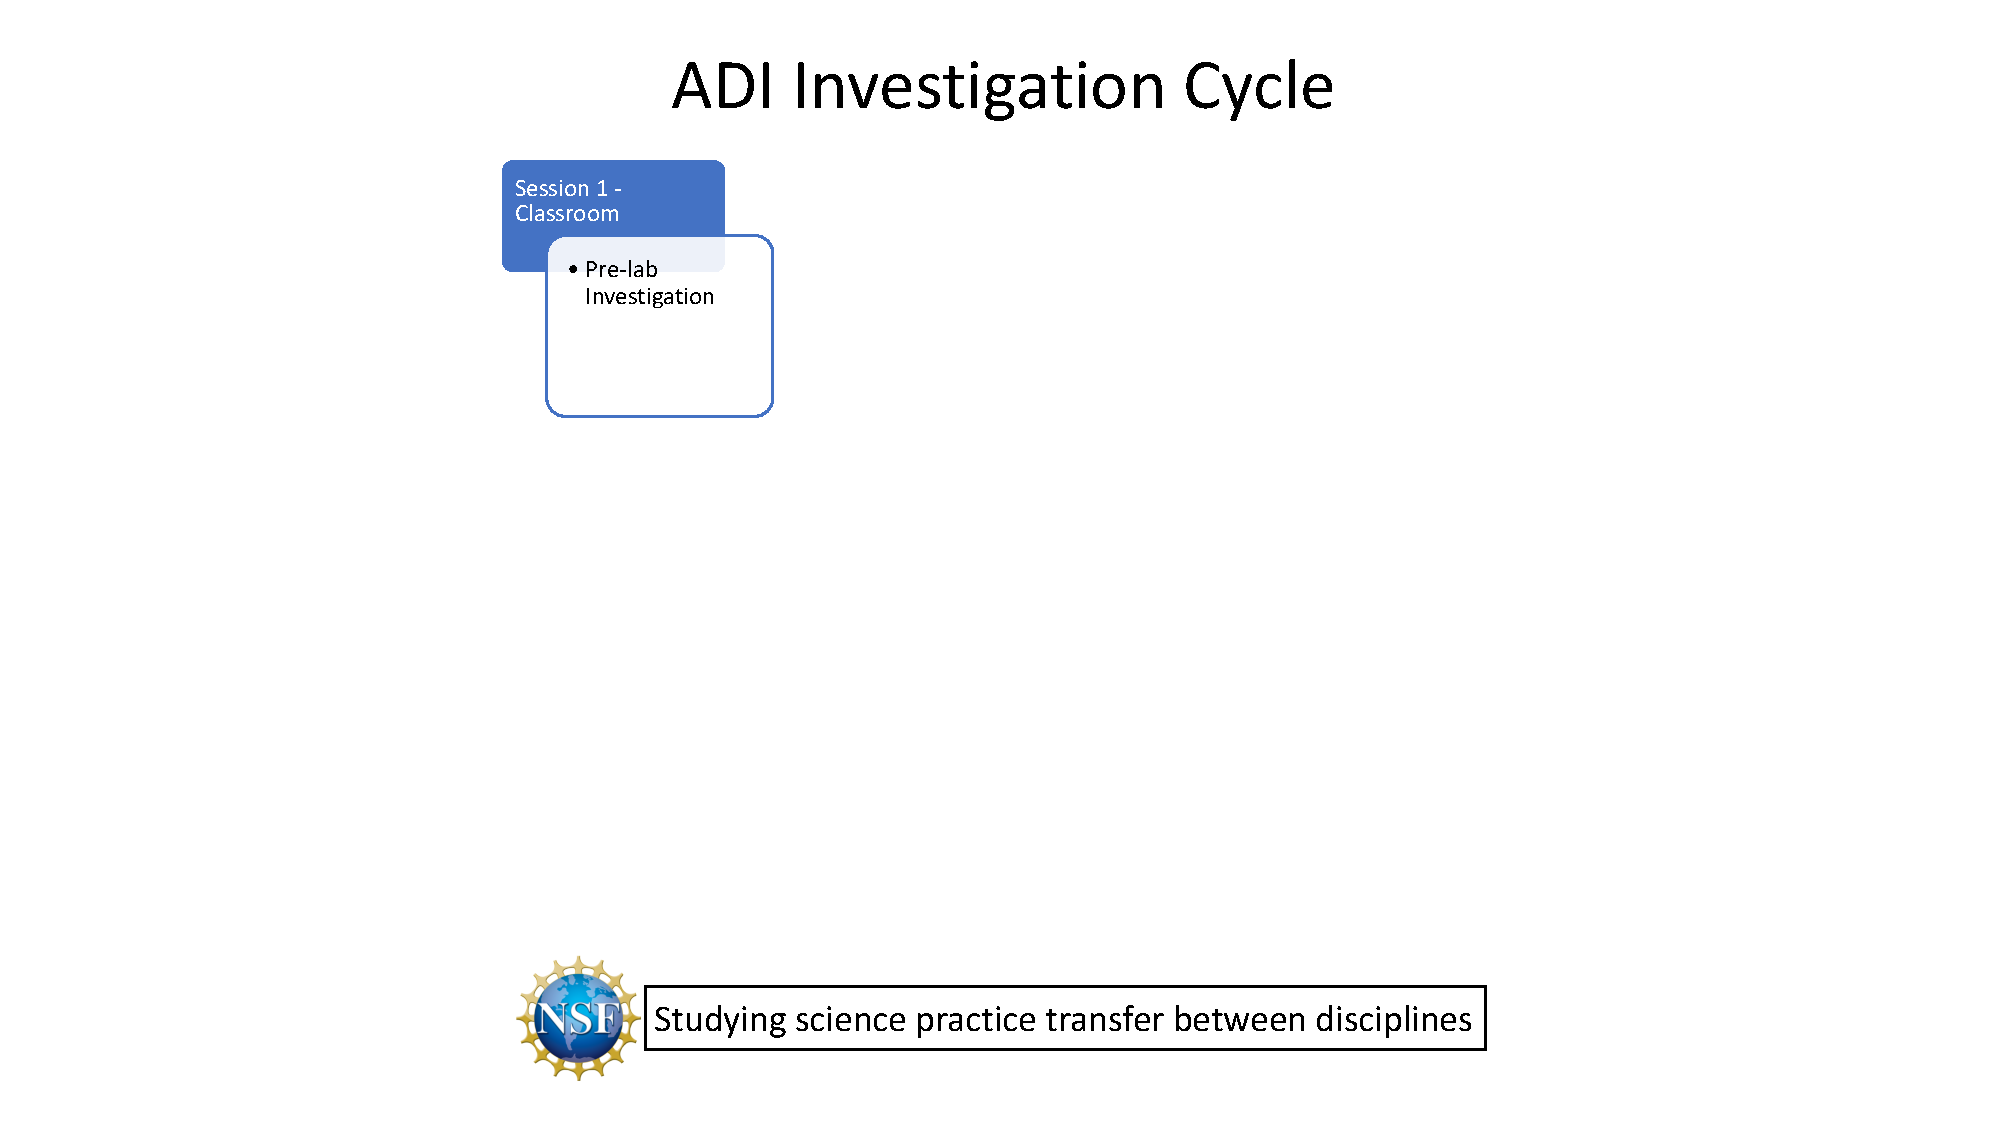
\includegraphics[page=1, height=3.in, valign=m]{PICUP1.pdf}}
\only<2>{\includegraphics[page=2, height=3in, valign=m]{PICUP1.pdf}}
\only<3>{\includegraphics[page=3, height=3in, valign=m]{PICUP1.pdf}}
\only<4>{\includegraphics[page=4, height=3in, valign=m]{PICUP1.pdf}}
\end{center}
\end{frame}

\begin{frame}
\frametitle{Change of plans: Labs are online now.}
\begin{center}
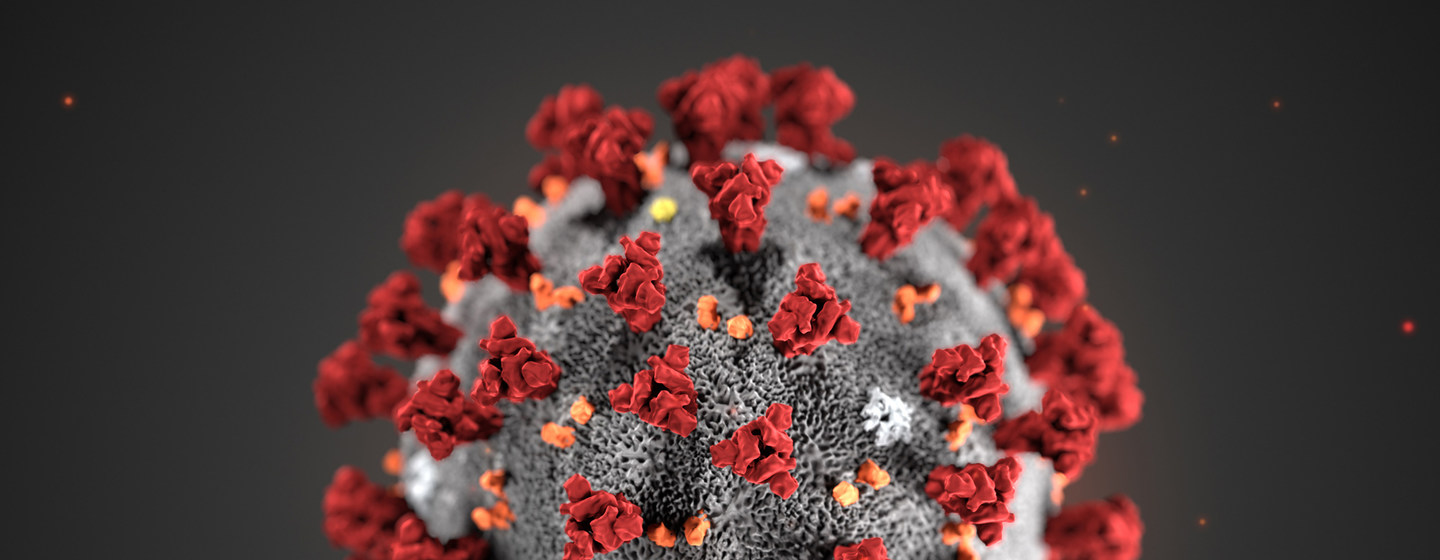
\includegraphics[width=2in]{coronavirus.jpg}
\end{center}
\begin{itemize}
\item<1-> Preserve ADI format for last two investigations
\item<2-> How can we change our delivery while maintaining our focus on science practices?
\item<3-> What do we need to do together?
\begin{enumerate}
\item Proposal approval
\item Argumentation session
\end{enumerate}
\item<4-> What can we do apart?
\begin{enumerate}
\item Data collection (Both Prelab and Inquiry Investigation)
\item Data analysis
\item Peer review/lab report revision
\end{enumerate}
\end{itemize}
\end{frame}

\begin{frame}
\frametitle{Implementing an ADI cycle--online delivery}
\begin{center}
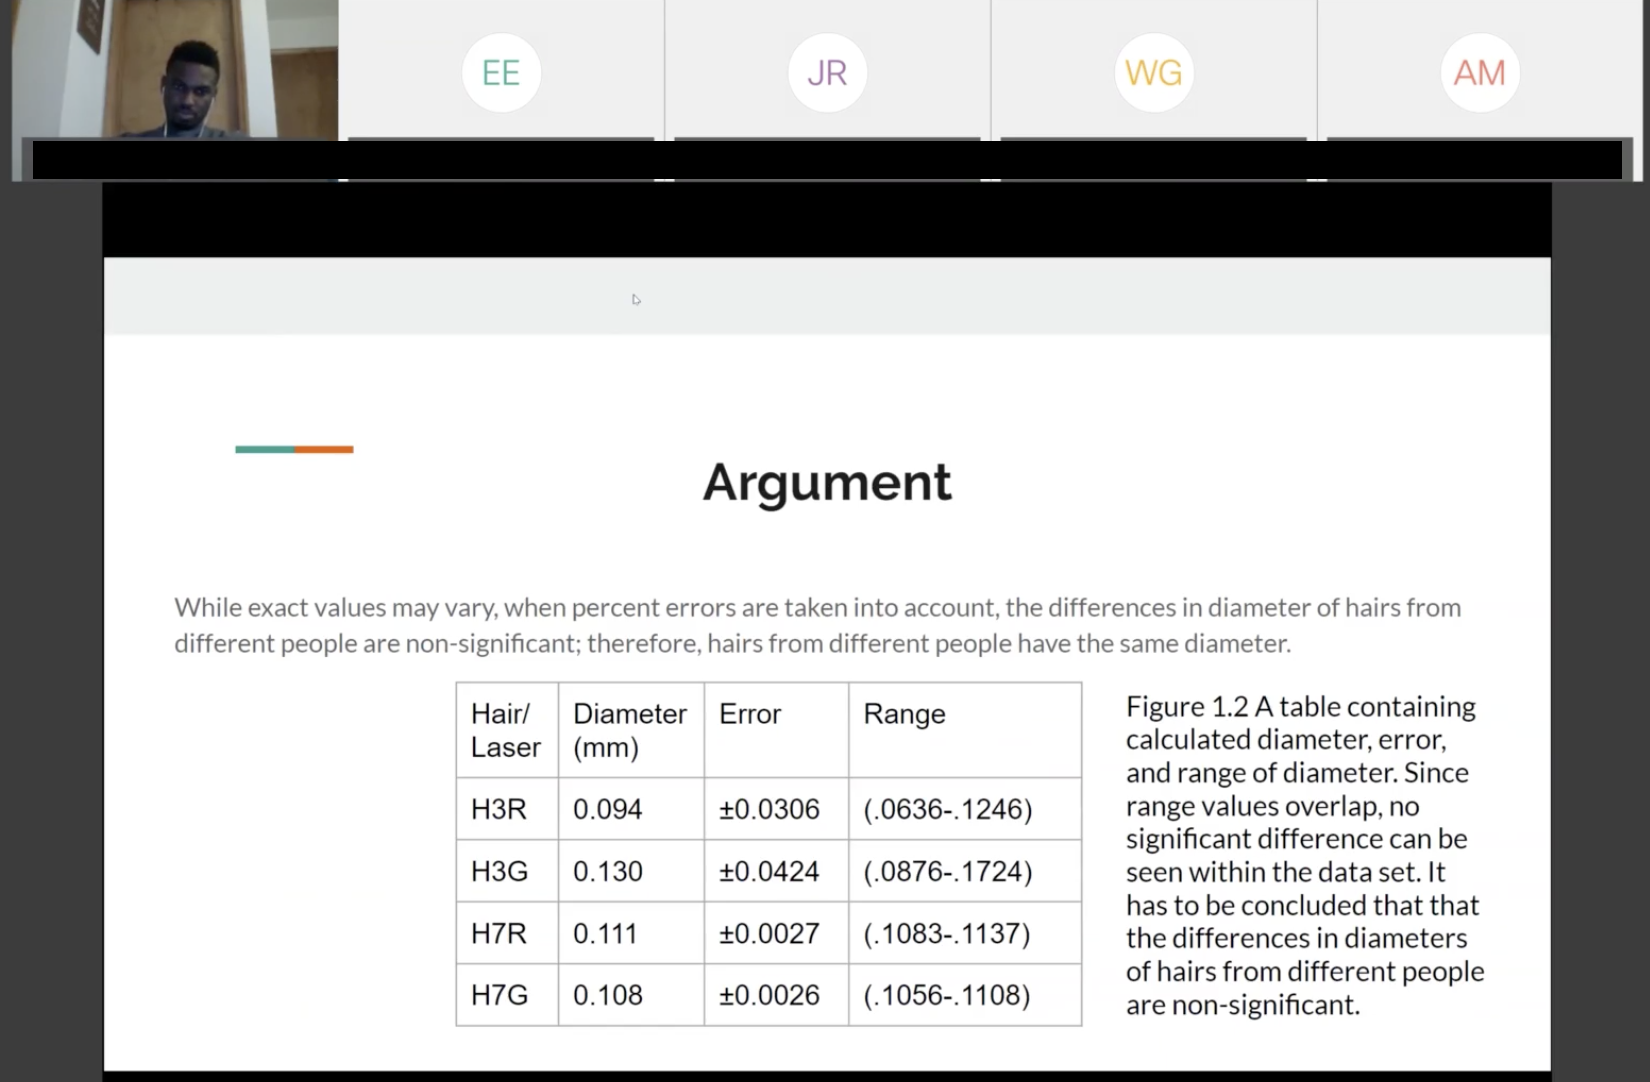
\includegraphics[width=2in]{WebExArgumentation.png}\\
{\footnotesize Student presentation in WebEx argumentation session.}
\end{center}
\begin{itemize}
\item<+-> Students complete pre-lab before proposal session
\item<+-> Proposal session--WebEx/Discussion Boards; approval by end of class time
\item<+-> Measurements/Analysis--Group completes before next lab session
\item<+-> Argumentation--3 slide PPT on WebEx during class time
\item<+-> Peer Review--asynchronous, online (same as in BC times)
\end{itemize}
\end{frame}

\begin{frame}
\frametitle{Measurements and Simulations}
\begin{center}
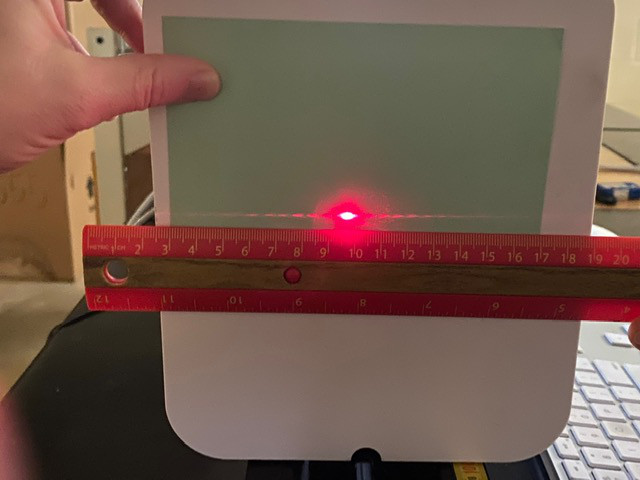
\includegraphics[width=2in]{Hair1_red_pattern.jpg}\\
{\footnotesize Image of diffraction pattern for student measurement.}
\end{center}
\begin{itemize}
\item Measurements online using photos and \href{run:Spring4_100g.mp4}{video}
\item Simulations on \emph{Trinket}
\end{itemize}
\end{frame}

%\begin{frame}
%\frametitle{Practical Exam and Beyond}
%
%\begin{tabular}{cc}
%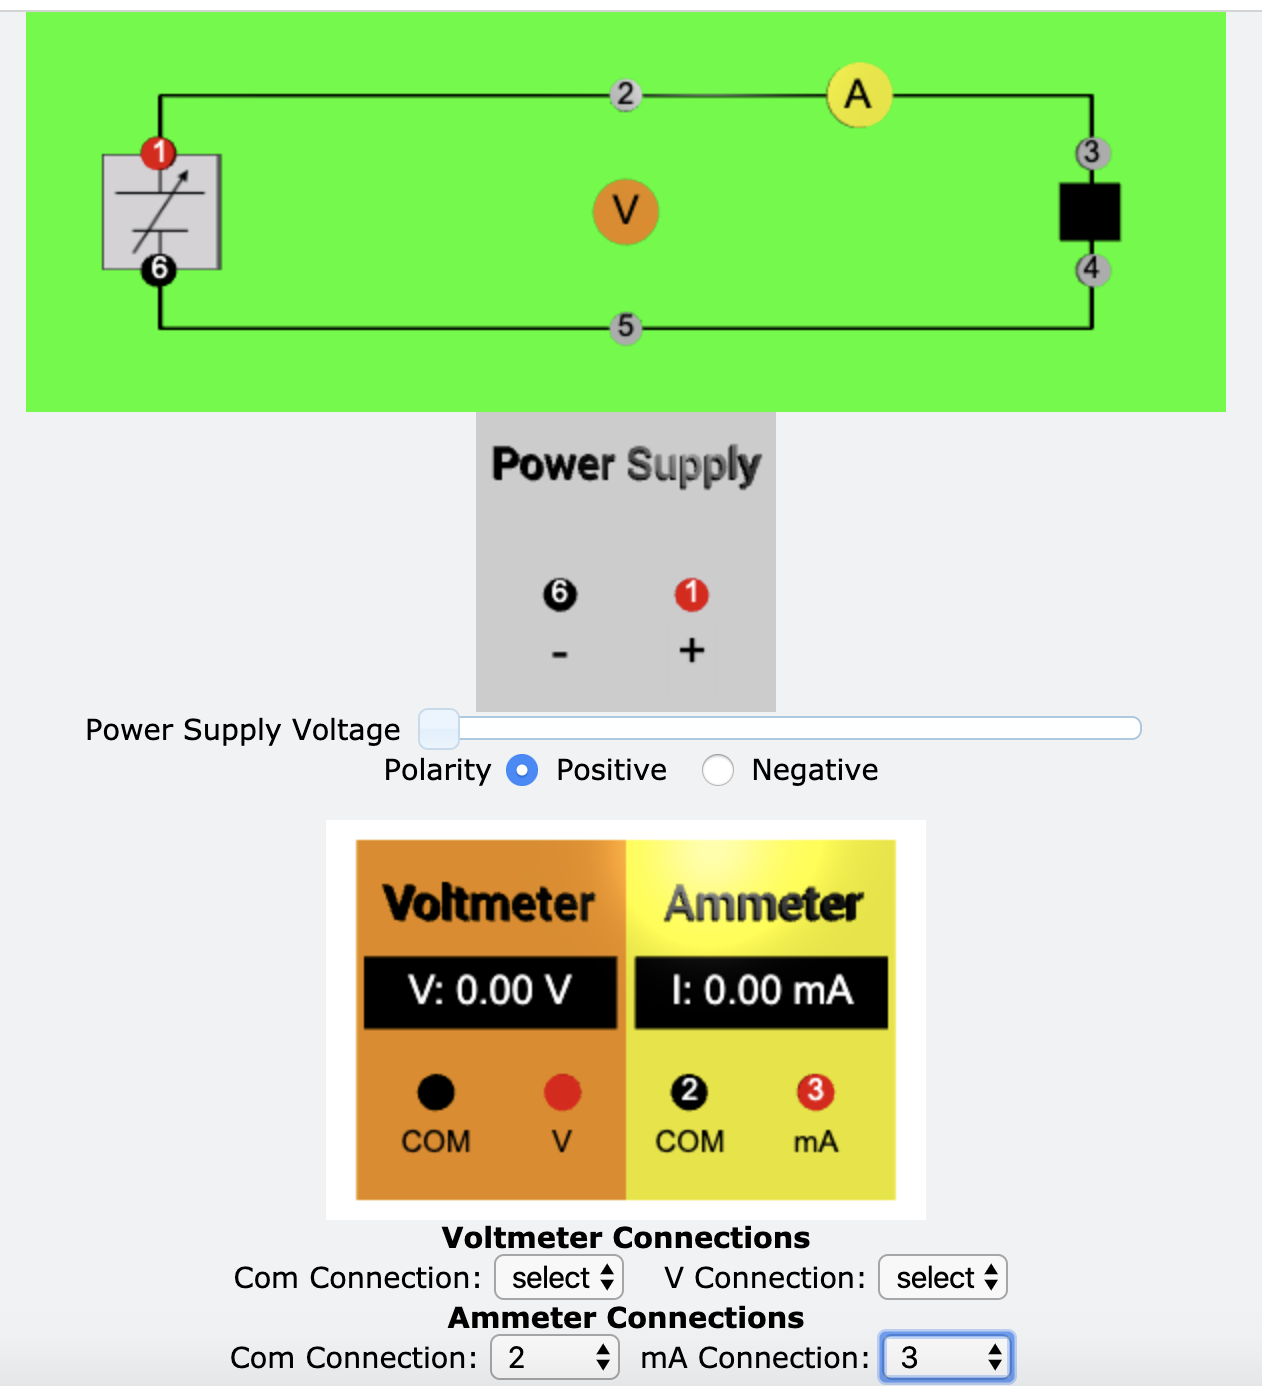
\includegraphics[width=2.5in, valign=m]{TrinketCircuit.png} &
%%
%\begin{minipage}[m]{0.5\linewidth}
%\begin{itemize}
%\uncover<1->{\item Practical exam
%\begin{itemize}
%\item Canvas quiz--different versions
%\item Measurements on Trinket simulation
%\item Analyze data and write argument
%\end{itemize}
%}
%
%\uncover<2->{\item Beyond
%\begin{itemize}
%\item Summer classes online (need new labs)
%\item Online lab sections after we emerge?
%\item Online lab make-ups?
%\end{itemize}
%}
%\end{itemize}
%
%\end{minipage}
%
%\end{tabular}
%
%\end{frame}

{\nologo
\begin{frame}
\frametitle{Tools used in online lab delivery}
\begin{center}
\renewcommand{\arraystretch}{1.5}
\begin{tabular}{cll}
\hline\hline
\textbf{Tool} & \textbf{Use} & \textbf{Rationale} \\
\hline
Canvas & \parbox[t]{2in}{\raggedright Material, Assignments, Quizzes, Discussions }& University LMS\\
WebEx & \parbox[t]{2in}{\raggedright Class introduction, argumentation, group interactions (???)} & University supported\\
Canvas & \parbox[t]{2in}{\raggedright Online peer review} & \parbox[t]{2in}{\raggedright Anonymous reviews and feedback}\\
Trinket.io & \parbox[t]{2in}{\raggedright Simulations embedded in Canvas} & Fine-grained control\\[3ex]
\hline\hline
\end{tabular}
\end{center}
\end{frame}
}

\end{document}